%=================================================================
\documentclass[commodities,article,submit,pdftex,moreauthors]{Definitions/mdpi}

\firstpage{1}
\makeatletter
\setcounter{page}{\@firstpage}
\makeatother
\pubvolume{1}
\issuenum{1}
\articlenumber{0}
\pubyear{2026}
\copyrightyear{2026}
\datereceived{ }
\daterevised{ }
\dateaccepted{ }
\datepublished{ }

\newcommand{\nConfigs}{1,568}
\newcommand{\evalStart}{2001-01-05}
\newcommand{\evalEnd}{2026-09-17}
\newcommand{\evalSessions}{6,469}
\newcommand{\evalYears}{25.7}
\newcommand{\holidays}{247}
\newcommand{\sessionsClean}{6,722}
\newcommand{\sessionsRaw}{6,969}
\newcommand{\clGeneric}{259.9\%}
\newcommand{\clTR}{46.0\%}
\newcommand{\ngGeneric}{$-$68.1\%}
\newcommand{\ngGenericAbs}{68.1\%}
\newcommand{\ngTRAbs}{99.98\%}
\newcommand{\ngTR}{$-$99.98\%}
\newcommand{\clNeg}{$-$37.63}
\newcommand{\liborLast}{2024-09-30}
\newcommand{\bhFinal}{206}
\newcommand{\bhCagr}{2.9\%}
\newcommand{\bhSharpe}{0.26}
\newcommand{\bhMdd}{$-$73.2\%}
\newcommand{\bhExSharpe}{0.15}
\newcommand{\refCorrLo}{0.83}
\newcommand{\refCorrHi}{0.91}
\newcommand{\ewSrLo}{0.26}
\newcommand{\ewSrHi}{0.33}
\newcommand{\beatTbillA}{81.6\%}
\newcommand{\beatBhA}{37.8\%}
\newcommand{\beatTbillB}{79.7\%}
\newcommand{\beatBhB}{35.3\%}
\newcommand{\beatTbillC}{77.5\%}
\newcommand{\beatBhC}{33.0\%}
\newcommand{\beatTbillD}{70.0\%}
\newcommand{\beatBhD}{27.1\%}
\newcommand{\bestGrossSr}{0.70}
\newcommand{\bestGrossFinal}{4,033}
\newcommand{\bestFinalGross}{5,117}
\newcommand{\bestFinalGrossSr}{0.67}
\newcommand{\bestFinalNetA}{2,143}
\newcommand{\bestFinalNetSrA}{0.61}
\newcommand{\bestFinalNetB}{2,137}
\newcommand{\bestFinalNetSrB}{0.61}
\newcommand{\bestFinalNetC}{2,118}
\newcommand{\bestFinalNetSrC}{0.61}
\newcommand{\rcP}{0.39}
\newcommand{\spaP}{0.02}
\newcommand{\spaT}{3.96}
\newcommand{\dsr}{0.63}
\newcommand{\dsrExpMax}{0.63}
\newcommand{\dsrSr}{0.70}
\newcommand{\pbo}{0.35}
\newcommand{\nDistinct}{1,372}
\newcommand{\dsrDistinct}{0.65}
\newcommand{\nDup}{196}
\newcommand{\pboComb}{12,870}
\newcommand{\volMedian}{21.8\%}
\newcommand{\volTop}{26.2\%}
\newcommand{\volWorst}{27.2\%}
\newcommand{\medBeatsEw}{67.9\%}
\newcommand{\topBeatsEw}{22.2\%}
\newcommand{\worstBeatsEw}{12.0\%}
\newcommand{\ngMedSixt}{19.4\%}
\newcommand{\ngMedNine}{17.2\%}
\newcommand{\goldMedNine}{44.0\%}
\newcommand{\exNgLo}{0.46}
\newcommand{\exNgHi}{0.58}
\newcommand{\exNgSix}{0.55 to 0.58}
\newcommand{\medMeanLo}{0.32}
\newcommand{\medMeanHi}{0.36}
\newcommand{\srTopMean}{0.20}
\newcommand{\srTopMax}{0.50}
\newcommand{\srMedMean}{0.34}
\newcommand{\srMedMax}{0.62}
\newcommand{\srWorMean}{0.16}
\newcommand{\srWorMax}{0.70}
\newcommand{\srTmwMean}{0.03}
\newcommand{\srTmwMax}{0.47}
\newcommand{\ncTop}{0}
\newcommand{\ncMed}{2}
\newcommand{\ncWor}{7}
\newcommand{\ncTmw}{0}
\newcommand{\revSrLo}{0.52}
\newcommand{\revSrHi}{0.70}
\newcommand{\revSrFiveLo}{$-$0.11}
\newcommand{\revSrFiveHi}{0.11}
\newcommand{\revSrOneLo}{0.39}
\newcommand{\revSrOneHi}{0.58}
\newcommand{\revSrTwoLo}{0.26}
\newcommand{\revSrTwoHi}{0.46}
\newcommand{\revTurnLo}{299}
\newcommand{\revTurnHi}{375}
\newcommand{\revBeBhLo}{2.2}
\newcommand{\revBeBhHi}{3.9}
\newcommand{\revBeCashLo}{3.6}
\newcommand{\revBeCashHi}{5.3}
\newcommand{\revNineLagZero}{0.67}
\newcommand{\revNineLagOne}{0.34}
\newcommand{\revSixLagZero}{0.61}
\newcommand{\revSixLagOne}{0.16}
\newcommand{\revUsLagZero}{0.55}
\newcommand{\revUsLagOne}{0.16}
\newcommand{\luckAnnRange}{0.42}
\newcommand{\luckSemiRange}{0.38}
\newcommand{\luckQRange}{0.15}
\newcommand{\luckAnnCalBest}{5.4\%}
\newcommand{\luckBwRange}{0.07}
\newcommand{\topAnnFirst}{6}
\newcommand{\topAnnWorstRank}{4}
\newcommand{\topAnnN}{10}
\newcommand{\starDec}{2,150}
\newcommand{\starMin}{115}
\newcommand{\starMaxOther}{1,302}
\newcommand{\starMedian}{416}
\newcommand{\starSrOtherMean}{0.33}
\newcommand{\starDecOne}{2,143}
\newcommand{\starMinOne}{115}
\newcommand{\starMaxOne}{1,297}
\newcommand{\bwGrid}{1,407}
\newcommand{\bwAlt}{389}
\newcommand{\bwAltSr}{0.35}
\newcommand{\starSrMin}{0.16}
\newcommand{\starSrMaxOther}{0.52}
\newcommand{\starSrMean}{0.36}
\newcommand{\starSrDec}{0.61}
\newcommand{\wfInLo}{0.86}
\newcommand{\wfInHi}{0.92}
\newcommand{\wfOutLo}{0.00}
\newcommand{\wfOutHi}{0.12}
\newcommand{\wfFinLo}{60}
\newcommand{\wfFinHi}{97}
\newcommand{\wfRankLo}{837}
\newcommand{\wfRankHi}{1,222}
\newcommand{\wfBhFinal}{149}
\newcommand{\wfBhSr}{0.29}
\newcommand{\wfMedOos}{0.14}
\newcommand{\wfaFinG}{135}
\newcommand{\wfaSrG}{0.19}
\newcommand{\wfaFinN}{47}
\newcommand{\wfaSrN}{0.02}
\newcommand{\wfaBh}{123}
\newcommand{\wfaBhSr}{0.14}
\newcommand{\wfaStart}{2006}
\newcommand{\scrDxLow}{64}
\newcommand{\scrDxHigh}{60}
\newcommand{\scrDxP}{0.79}
\newcommand{\scrFreeLow}{204}
\newcommand{\scrFreeHigh}{82}
\newcommand{\scrNBloom}{30}
\newcommand{\scrNFail}{9}
\newcommand{\turnDaily}{128}
\newcommand{\turnAnnual}{1.3}
\newcommand{\nBeatDaily}{102}
\newcommand{\nBeatAnnual}{64}
\newcommand{\lmePreLo}{20}
\newcommand{\lmePreHi}{27}
\newcommand{\kwPre}{3.3}
\newcommand{\nNoiseClose}{3}
\newcommand{\ncMedW}{two}
\newcommand{\ncWorW}{seven}
\newcommand{\nNoiseCloseW}{Three}
\newcommand{\beMedDaily}{2.2}
\newcommand{\beMedAnnual}{234}


%=================================================================
\Title{Volatility Sorting, an Untradeable Reversal and Rebalance-Date Luck: What Survives a Declared Search Over Cross-Sectional Commodity Strategies}

\newcommand{\orcidauthorA}{0009-0005-6739-8265}

\Author{Aryan Meena $^{1}$\orcidA{} and Eugene Pinsky $^{1,}$*}

\AuthorNames{Aryan Meena and Eugene Pinsky}

\address{%
$^{1}$ \quad Department of Computer Science, Metropolitan College, Boston University, 1010 Commonwealth Avenue, Boston, MA 02215, USA; aryan18@bu.edu (A.M.); epinsky@bu.edu (E.P.)}

\corres{Correspondence: epinsky@bu.edu}

%=================================================================
\abstract{Cross-sectional commodity strategies are usually tested one specification at a time, which hides how many were tried. We declare the whole search. On Bloomberg Commodity Index total-return sub-indices for the six to nine most liquid commodities, we rank assets by trailing return, split them into best, middle and worst groups, and evaluate \nConfigs{} configurations spanning seven lookbacks, seven rebalance frequencies and eight universe splits from January 2001 to September 2026. Each grid is compared with a noise ceiling, the best Sharpe ratio the same search attains with random rankings. Three results look promising, yet none is an edge an investor could have exploited. The middle group beats equal weighting in \medBeatsEw{} of cells, mostly by holding the most volatile commodities less often. A one-day reversal is statistically real (Hansen's superior predictive ability test, $p \approx \spaP$) but vanishes with a one-session execution delay and near 5 basis points of cost. The best net-of-cost configuration, an annual rebalance, depends on its rebalance date: the same rule rebalanced at other month-ends finishes with USD \starMin{} to USD \starMaxOther{} instead of USD \starDec. The top configurations by Sharpe ratio over 2001--2013 all trail buy-and-hold over 2014--2026, and momentum never exceeds its noise ceiling.}

\keyword{commodity futures; cross-sectional momentum; short-term reversal; backtest overfitting; data snooping; rebalance timing luck; transaction costs; Bloomberg Commodity Index}

\JEL{C12; C15; G11; G13; G14; Q02}

%=================================================================
\begin{document}

\section{Introduction}

A commodity investor who ranks a handful of liquid markets by their recent performance and holds some of them has to make at least five choices before a single return is computed: which commodities, how far back to measure performance, how often to rebalance, which part of the ranking to hold, and on which date to rebalance. The published literature typically reports grids of formation and holding periods without adjusting for the search, on generic front-month price series and over broad universes of twenty or more contracts \citep{miffre2007,shen2007,fuertes2010,zhang2020}. A parallel literature shows that searching over specifications inflates backtested performance, and that the correction must account for everything that was tried \citep{sullivan1999,white2000,hansen2005,romano2005,bailey2014,harvey2016}.

This paper brings the two strands together for the small, investable universe that practitioners actually trade. We take the six to nine most liquid commodities in a Bloomberg terminal pull, use the Bloomberg Commodity Index (BCOM) total-return sub-indices that an investor holding and rolling the futures would earn, and declare the full search: seven lookbacks from one day to one year, seven rebalance frequencies from daily to annual, three ranked groups plus the long--short spread, and eight ways of splitting the universe into groups. That is \nConfigs{} configurations, each evaluated gross and net of costs over \evalYears{} years. Rather than report the winner, we ask which results survive four tests that a careful investor would apply before committing capital: a noise ceiling built by rerunning the whole search with random rankings, formal multiple-testing corrections, a realistic execution delay, and out-of-sample selection.

Our contribution is a set of negative results, each accompanied by an explanation of why it arises. First, cross-sectional momentum does not survive: no momentum spread in any universe exceeds its noise ceiling. Second, the middle group, the portfolio that holds neither recent winners nor recent losers, beats equal weighting in most of the grid, but the reason is mechanical. The most volatile commodities are the most likely to sit at the extremes of any ranking, so the middle group holds them less often. Natural gas, which lost \ngTRAbs{} of its value in total-return terms over the sample, sits in the middle group less than 20\% of the time against one third under a random ranking. Third, a one-day reversal (holding yesterday's worst performers) is the only effect that clears both the noise ceiling and the Hansen test of superior predictive ability. It vanishes, however, if the trade is placed one session after the signal, and at about 5 basis points (bp) it costs more to trade than it earns. Fourth, the configuration that ranks first net of costs, an annual rebalance of the middle group, owes much of its rank to the calendar. Rebalanced at other month-ends, the same rule produces a fraction of the result, which is the rebalance-date luck previously documented for fixed-mix and equity factor portfolios \citep{hoffstein2019,hoffstein2020}.

The closest precedent, published in this journal, reports momentum terciles for commodity futures without multiple-testing correction \citep{adhikari2024}. We extend it by treating the middle tercile as the object of study, benchmarking an entire configuration search against randomised rankings, and adding costs, execution delay, rebalance-date sensitivity and out-of-sample selection. The results complement a companion study of the U.S. Dollar Index (DXY) \citep{meena2026}, which documents how a data defect and an undeclared search can each manufacture a convincing backtest. In the present study the data are clean and the search is declared, and the same discipline still removes every candidate edge.

Section~\ref{sec:lit} reviews the literature. Section~\ref{sec:data} describes the data, the choice of total-return sub-indices over generic futures prices, the strategies and the tests. Section~\ref{sec:results} reports the results and Section~\ref{sec:discussion} discusses their implications and limitations.

\section{Related Literature}\label{sec:lit}

\subsection{Cross-Sectional Commodity Premia}

Commodity futures earn premia related to the shape of the futures curve, hedging pressure and past returns \citep{erb2006,gorton2006,gorton2013,szymanowska2014}. Cross-sectional momentum, buying the recent best performers and selling the worst, has been documented by \citet{miffre2007} and \citet{shen2007}, and combined with term-structure signals by \citet{fuertes2010}; \citet{szakmary2010} document time-series trend-following profits in 28 commodity futures, and \citet{zhang2020} find significant momentum and no reversal profits across 189 formation and holding windows. Factor models of the commodity cross-section include \citet{bakshi2019} and \citet{daskalaki2014}; momentum across asset classes is studied by \citet{asness2013} and time-series momentum by \citet{moskowitz2012}. Most of this evidence comes from universes of twenty or more contracts and from long--short portfolios of the extreme groups. \citet{adhikari2024} reports high, medium and low momentum terciles for 29 commodity futures at one-, three- and twelve-month lookbacks with monthly rebalancing and no lag, without correcting for multiple testing or costs.

\subsection{Short-Term Reversal}

In equities, returns over the previous week or month partly reverse \citep{jegadeesh1990,lehmann1990}. In futures markets, \citet{wang2004} find weekly reversal across 24 US futures, and \citet{kang2020} show, using trader positions, that weekly changes in speculators' positions predict subsequent returns with the opposite sign, compensating hedgers for providing liquidity. \citet{dellacorte2015} report that the daily close-to-close reversal is negative, that is, daily momentum, in 11 mostly agricultural and livestock futures. \citet{bianchi2015} study longer-horizon reversal combined with momentum. We add a daily horizon on investable total-return indices, and test whether the effect survives an execution delay.

\subsection{Searching over Specifications}

White's Reality Check \citep{white2000}, Hansen's test of superior predictive ability \citep{hansen2005} and the stepwise procedure of \citet{romano2005} control the probability that the best of many strategies looks good by chance; \citet{sullivan1999} apply the Reality Check to technical trading rules. The deflated Sharpe ratio \citep{bailey2014} and the probability of backtest overfitting \citep{bailey2017} measure the same risk from the Sharpe ratios of the trials. \citet{harvey2016} and \citet{harvey2015} argue for much higher significance thresholds in finance, and \citet{mclean2016} show that published anomalies weaken after publication. In commodities, \citet{marshall2008} evaluate more than 7,000 technical rules on 15 futures with a bootstrap adjustment for data snooping and find no consistent profitability, and \citet{psaradellis2023} apply false-discovery-rate control to technical rules on commodity, equity and currency spreads and find commodity spreads predictable. The noise ceiling used here is a direct, strategy-specific counterpart to these tests, in the spirit of random-portfolio benchmarks \citep{arnott2013} and of large-scale comparisons with data-mined strategies \citep{chordia2020}: it reruns the exact search with the information in the ranking destroyed.

\subsection{Implementation}

Trading costs remove a large share of published anomaly returns \citep{novymarx2016}, and commodity futures have their own cost structure \citep{marshall2012}. The roll method and position on the futures curve materially change commodity index and strategy returns \citep{mouakhar2010,degroot2014}, which is one reason we use standardised total-return sub-indices. \citet{hoffstein2019} show that the rebalance date alone changes the realised returns of fixed-mix portfolios, and \citet{hoffstein2020} that for equity smart-beta factor indices the dispersion across rebalance dates often exceeds one percentage point a year; we are not aware of a comparable study for commodity cross-sectional rules. Finally, \citet{demiguel2009} show that simple equal weighting is hard to beat out of sample, which motivates using it as the fair benchmark for every group.

\section{Materials and Methods}\label{sec:data}

\subsection{Data Source}

All data were retrieved from a Bloomberg terminal at Boston University in September 2026 and cover 2000-01-03 to 2026-09-17 (\sessionsRaw{} weekday rows). The pull has three parts: total-return indices for 28 BCOM single-commodity sub-indices; the generic first contract (open, high, low, last, aggregate volume and open interest) for 30 commodity futures; and the BCOM total-return index (BCOMTR), the three-month USD London Interbank Offered Rate (LIBOR) and the S\&P 500. BCOM sub-indices roll from the lead future into the next designated contract over the sixth to tenth business days of the month and are fully collateralised with Treasury bills \citep{bloomberg2023bcom}, so their total return is what a fully collateralised investor holding the futures would have earned.

\subsection{Total-Return Sub-Indices Rather Than Generic Futures Prices}

A generic first-contract series splices consecutive contracts together. Each splice is a price difference between two contracts and not a return anyone earns, and a percentage return is undefined when the price is negative, as the generic West Texas Intermediate (WTI) crude oil contract was on 2020-04-20 (USD \clNeg). The difference is large. From the start of our evaluation window, the generic WTI price rose \clGeneric{} while the WTI total-return sub-index rose \clTR; the generic natural gas price fell \ngGenericAbs{} while its total-return sub-index fell \ngTRAbs{} (Figure~\ref{fig:tr}). Ranking commodities on generic prices would therefore rank them on returns that no investor could have earned, so we use the generic contracts only to measure liquidity.

\begin{figure}[H]
\begin{adjustwidth}{-\extralength}{0cm}
\centering
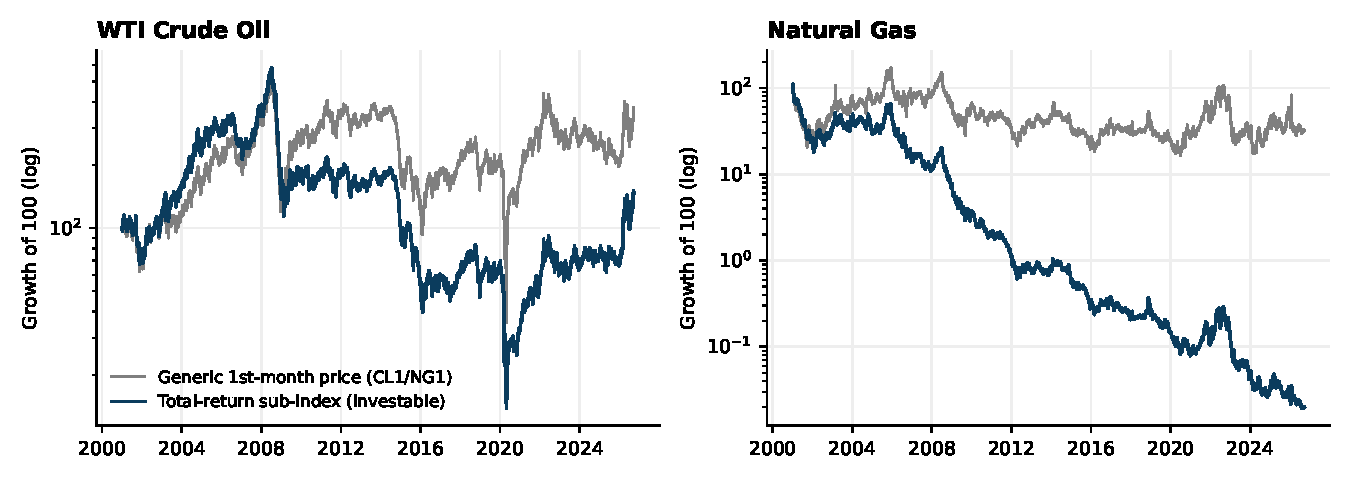
\includegraphics[width=\linewidth]{figs/fig1_generic_vs_tr.pdf}
\caption{Growth of 100 invested at the start of the evaluation window: the generic first-month futures price against the BCOM total-return sub-index for WTI crude oil and natural gas (log scale). The gap is roll yield and collateral return; the WTI generic series is not shown where its price was negative.\label{fig:tr}}
\end{adjustwidth}
\end{figure}

\subsection{Cleaning}

The three sheets share a Monday-to-Friday calendar with holidays filled forward. We drop the \holidays{} sessions on which all 28 sub-indices are unchanged from the previous session, leaving \sessionsClean{} sessions; no other values are missing. The LIBOR series stops changing on \liborLast{} after the cessation of USD LIBOR, so we use the three-month Treasury bill rate from the Federal Reserve Economic Data service (FRED, series DTB3) as the risk-free rate.

\subsection{Universe}

We rank the 30 generic contracts by mean daily notional volume (price times aggregate volume times contract multiplier) over 2000--2026 and, separately, by notional open interest over the last twelve months. Three refined products, RBOB gasoline, heating oil and gasoil, are excluded because their weekly returns have correlations of \refCorrLo{} to \refCorrHi{} with WTI and Brent, so including them would largely duplicate crude oil. Palladium and orange juice have no total-return sub-index in the pull. Ordering the remaining contracts by the average of their two ranks, the nine most liquid commodities form four nested universes (Table~\ref{tab:assets}): Top6 (WTI, Brent, gold, natural gas, soybeans, silver) and Top7, Top8 and Top9, which add aluminium, corn and copper in turn. Because liquidity is measured over the whole sample, the universe is chosen with some hindsight (copper, for example, was less liquid in the early 2000s than it later became); we return to this point in Section~\ref{sec:limits}.

\begin{table}[H]
\begin{adjustwidth}{-\extralength}{0cm}
\caption{The traded universe. Liquidity ranks are among the 30 generic contracts in the Bloomberg pull, by mean daily notional volume over 2000--2026 (Vol.) and by mean notional open interest over the last twelve months (OI); the universe is ordered by the average of the two ranks. Return statistics use the total-return sub-index over \evalStart{} to \evalEnd{}.\label{tab:assets}}
\small
\begin{tabularx}{\fulllength}{lllrrrrrr}
\toprule
\textbf{Universe} & \textbf{Commodity} & \textbf{Sub-index} & \textbf{Vol.} & \textbf{OI} & \textbf{CAGR} & \textbf{Volatility} & \textbf{Sharpe} & \textbf{Max DD}\\
\midrule
Top6 & WTI Crude Oil & BCOMCLTR & 1 & 3 & 1.5\% & 38.4\% & 0.23 & $-$97.6\%\\
Top6 & Brent Crude Oil & BCOMCOT & 2 & 1 & 8.5\% & 34.4\% & 0.41 & $-$90.7\%\\
Top6 & Gold & BCOMGCTR & 3 & 2 & 10.6\% & 17.9\% & 0.65 & $-$45.7\%\\
Top6 & Natural Gas & BCOMNGTR & 7 & 6 & $-$28.2\% & 49.0\% & $-$0.43 & $-$99.98\%\\
Top6 & Soybeans & BCOMSYTR & 8 & 5 & 7.6\% & 22.5\% & 0.44 & $-$52.5\%\\
Top6 & Silver & BCOMSITR & 10 & 7 & 9.8\% & 33.2\% & 0.45 & $-$78.2\%\\
+Top7 & Aluminium & BCOMALTR & 9 & 10 & 0.9\% & 21.3\% & 0.15 & $-$74.8\%\\
+Top8 & Corn & BCOMCNTR & 11 & 11 & $-$4.1\% & 26.0\% & $-$0.03 & $-$81.5\%\\
+Top9 & Copper & BCOMHGTR & 12 & 12 & 8.9\% & 26.9\% & 0.45 & $-$68.5\%\\
\midrule
 & BCOMTR (benchmark) & BCOMTR & -- & -- & 2.9\% & 16.2\% & 0.26 & $-$73.2\%\\
\bottomrule
\end{tabularx}
\end{adjustwidth}
\end{table}



\subsection{Strategies}\label{sec:method}

At each rebalance session $s$, commodity $i$ is ranked by its trailing total return $P_i(s)/P_i(s-L)-1$ over a lookback of $L$ sessions, using only prices up to and including the close of $s$. The ranking is split into three groups: the best $k_1$ performers (Top), the next $k_2$ (Median) and the worst $k_3$ (Worst). Each group is bought at equal weight at the close of $s$ and held, with weights drifting with prices, until the next rebalance; the first return a new portfolio earns is from the close of $s$ to the close of $s+1$. We also report the long--short spread Top minus Worst, the classic cross-sectional momentum portfolio.

The grid comprises seven lookbacks, $L \in \{1, 5, 10, 21, 63, 126, 252\}$ sessions; seven rebalance frequencies (daily; weekly on Fridays; biweekly on every second Friday; monthly; quarterly; semiannually in June and December; annually at year-end); and eight group splits: 2-2-2 for Top6, 3-2-2, 2-3-2 and 2-2-3 for Top7, 3-3-2, 3-2-3 and 2-3-3 for Top8, and 3-3-3 for Top9. With four portfolios per cell this gives $8 \times 7 \times 7 \times 4 = \nConfigs$ configurations. Weekly rebalances fall on the last session of each week (a Friday unless it is a holiday) and biweekly rebalances on alternate week-ends, counted from the second week-end after the start; monthly, quarterly, semiannual and annual rebalances fall on the last session of the period. Every configuration first rebalances on 2001-01-04, the first session for which a 252-session lookback exists, so all are evaluated on the same \evalSessions{} sessions from \evalStart{} to \evalEnd. Because extreme groups can coincide across splits (the Top group of Top7 holds the best two commodities under both the 2-3-2 and 2-2-3 splits, for example), \nDup{} configurations duplicate another exactly, leaving \nDistinct{} distinct portfolios; we keep the full grid so that every split is reported symmetrically.

\subsection{Benchmarks, Costs and Metrics}

We compare every configuration with BCOMTR buy-and-hold and with 1/N, the equal-weighted portfolio of the same commodities rebalanced at the same frequency \citep{demiguel2009}. Transaction costs are charged at $c$ bp per unit of one-way turnover on the first session of each holding period, where turnover is the sum of absolute differences between the target weights and the drifted weights; the initial purchase counts as a turnover of one. Because this cost model is linear in $c$, one gross run of each configuration gives its exact net result at every cost level, and we compute the break-even cost at which a configuration's terminal value equals that of buy-and-hold. The long--short spread pays costs on both legs.

Sharpe ratios are annualised from daily returns with $\sqrt{252}$ at a zero risk-free rate, as in the companion DXY study; excess-of-bill Sharpe ratios subtract the daily Treasury bill accrual (except for the self-financing spread). We also report the compound annual growth rate (CAGR), maximum drawdown and the terminal value of USD 100.

\subsection{Noise Ceiling}

For each universe split we rerun the entire 49-cell grid (seven lookbacks by seven frequencies) with the ranking at every rebalance replaced by a random permutation. The commodity returns, rebalance calendars, group sizes and holding rules are left unchanged, so the only thing removed is the information in past returns. We record the best Sharpe ratio in the grid for each portfolio type, repeat 200 times, and call the 95th percentile of that best-of-49 distribution the noise ceiling. A real configuration that falls below its ceiling cannot be distinguished from what a search of this size produces with no signal at all.

\subsection{Formal Multiple-Testing Diagnostics}

Across all \nConfigs{} configurations we compute White's Reality Check and Hansen's consistent test of superior predictive ability (SPA), with the stationary bootstrap of \citet{politis1994} (mean block length 21 sessions, 5000 replications) applied jointly to all configurations. Performance is measured against 1/N of the same commodities at the same frequency for the long-only groups and against zero for the long--short spread. We also report the deflated Sharpe ratio of the best configuration \citep{bailey2014}, with the number of trials set to \nConfigs{} (and, as a check, to the \nDistinct{} distinct portfolios), and the probability of backtest overfitting from combinatorially symmetric cross-validation (CSCV) with 16 blocks \citep{bailey2017}.

\subsection{Implementation Checks}

Three further checks address the specific ways in which a configuration can look better in a backtest than it would in practice. The \emph{execution delay} test holds the portfolio chosen at the close of $s$ from the close of $s+1$ instead, as an investor who learns the closing prices after the close would. The \emph{rebalance-date} test reruns every quarterly, semiannual and annual configuration with each possible month-end offset (three, six and twelve offsets respectively), and every biweekly configuration on the other set of alternate weeks, and records the spread of Sharpe ratios across offsets. The \emph{out-of-sample} test selects the five configurations with the highest gross Sharpe ratio over 2001--2013 and runs them unchanged over 2014--2026. An expanding-window variant selects the best configuration at the end of each year, starting at the end of 2005, and holds it for the following year. Its net-of-cost version selects on net Sharpe ratios and ignores the cost of switching between configurations.

\subsection{Software}

All computations were carried out in Python with NumPy, pandas, SciPy and Matplotlib. Every number, table and figure is generated directly from the code, and a second, independently written implementation of the backtest reproduced the results of all \nConfigs{} configurations to numerical precision. The use of generative AI tools is described in the Acknowledgments.

\section{Results}\label{sec:results}

\subsection{Overview}

Table~\ref{tab:assets} shows how much the nine commodities differ. Gold has the highest Sharpe ratio of the nine and natural gas the lowest, with a total-return loss of 28\% a year. BCOMTR buy-and-hold turns USD 100 into USD \bhFinal{} (Sharpe \bhSharpe, maximum drawdown \bhMdd), and 1/N portfolios of the universes reach Sharpe ratios of \ewSrLo{} to \ewSrHi.

Across the grid, the middle group has the highest mean Sharpe ratio (\srMedMean{} against \srTopMean{} for Top, \srWorMean{} for Worst and \srTmwMean{} for the momentum spread). Before costs, \beatTbillA{} of configurations beat Treasury bills and \beatBhA{} end above buy-and-hold; at 5 bp these shares fall to \beatTbillD{} and \beatBhD. Table~\ref{tab:bestfreq} and Figure~\ref{fig:bestfreq} show the configuration with the highest gross terminal value at each rebalance frequency. The daily winner, holding the two worst performers of the previous session, turns USD 100 into USD \bestFinalGross{} before costs, but a cost of only \revBeBhLo{} to \revBeBhHi{} bp per unit of turnover would bring the daily reversal configurations down to buy-and-hold. At the other end, the best annual configuration, the middle two of Top6 with a 21-session lookback, is almost insensitive to cost: USD \bestFinalNetA{} at 1 bp and USD \bestFinalNetC{} at 5 bp, and it ranks first by terminal value at every cost from 1 to 5 bp. Mean turnover of the long-only groups falls from \turnDaily{} times a year for daily rebalancing to \turnAnnual{} for annual, and among the configurations that beat buy-and-hold before costs (\nBeatDaily{} of 224 daily and \nBeatAnnual{} of 224 annual), the median break-even cost rises from \beMedDaily{} bp to \beMedAnnual{} bp.

\begin{table}[H]
\begin{adjustwidth}{-\extralength}{0cm}
\caption{Best configuration at each rebalance frequency (highest gross terminal value), with the terminal value of USD 100 net of 0, 1, 2 and 5 bp per unit of one-way turnover, and the cost at which it would end level with BCOMTR buy-and-hold (USD \bhFinal).\label{tab:bestfreq}}
\small
\begin{tabularx}{\fulllength}{lXrrrrrrr}
\toprule
\textbf{Rebalance} & \textbf{Configuration} & \textbf{Turn./yr} & \textbf{0 bp} & \textbf{1 bp} & \textbf{2 bp} & \textbf{5 bp} & \textbf{Sharpe} & \textbf{Break-even (bp)}\\
\midrule
Daily & Worst 2 of 7 (3-2-2), 1d & 360.1 & 5,117 & 2,031 & 806 & 50 & 0.67 & 3.5\\
Weekly & Middle 3 of 9 (3-3-3), 10d & 61.7 & 1,379 & 1,177 & 1,005 & 625 & 0.62 & 12.0\\
Biweekly & Middle 2 of 7 (2-2-3), 10d & 36.4 & 1,407 & 1,282 & 1,168 & 882 & 0.56 & 20.5\\
Monthly & Middle 2 of 7 (2-2-3), 21d & 15.9 & 805 & 772 & 741 & 656 & 0.48 & 33.2\\
Quarterly & Middle 2 of 6 (2-2-2), 5d & 5.2 & 1,308 & 1,291 & 1,274 & 1,225 & 0.52 & 138.5\\
Semiannual & Middle 2 of 7 (3-2-2), 252d & 2.8 & 1,396 & 1,386 & 1,376 & 1,347 & 0.56 & 262.5\\
Annual & Middle 2 of 6 (2-2-2), 21d & 1.2 & 2,150 & 2,143 & 2,137 & 2,118 & 0.61 & 738.9\\
\bottomrule
\end{tabularx}
\end{adjustwidth}
\end{table}



\begin{figure}[H]
\begin{adjustwidth}{-\extralength}{0cm}
\centering
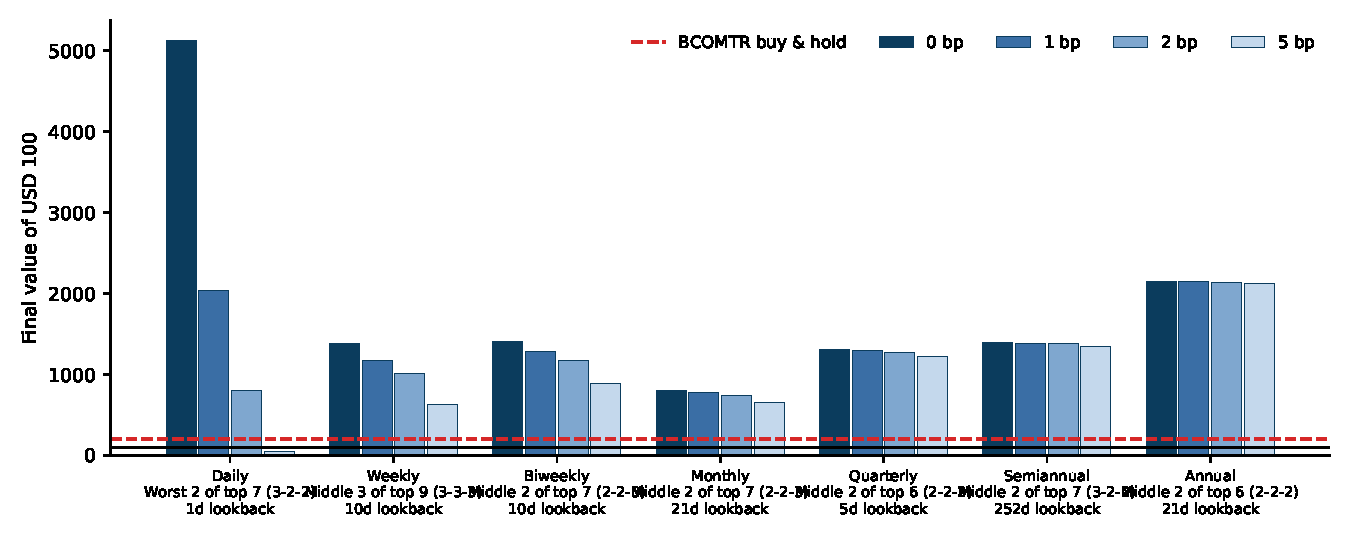
\includegraphics[width=\linewidth]{figs/fig3_best_per_frequency.pdf}
\caption{Terminal value of USD 100 for the best configuration at each rebalance frequency, at 0, 1, 2 and 5 bp per unit of turnover. The dashed line is BCOMTR buy-and-hold. The replication notebook produces the same chart for the top five configurations at each frequency and for maximum drawdown.\label{fig:bestfreq}}
\end{adjustwidth}
\end{figure}

Taken at face value, Table~\ref{tab:bestfreq} suggests that several configurations beat the benchmark by a wide margin even after costs. The remainder of this section asks whether any of them would have been found, and would have worked, without the benefit of hindsight.

\subsection{Noise Ceiling and Formal Tests}

Table~\ref{tab:noise} and Figure~\ref{fig:noise} compare the best configuration in each 49-cell grid with its noise ceiling. The momentum spread never exceeds its ceiling, and its best Sharpe ratio sits close to the median of the random-ranking best, so a search of this size produces spreads as good as the real ones from rankings that carry no information. The Top group never exceeds its ceiling either. The Median group exceeds it in \ncMedW{} of the eight grids and the Worst group in \ncWorW{}; every Worst exceedance, and one of the two Median exceedances, is the one-day lookback with daily rebalancing, examined in Section~\ref{sec:reversal}. \nNoiseCloseW{} verdicts, marked with a dagger in Table~\ref{tab:noise}, lie within 0.01 of the ceiling and are within simulation error: the Top6 middle group, which contains the best net-of-cost configuration, the Top6 worst group and the Top7 2-3-2 middle group. A different random seed could move any of them across the line, so none should be read as clearly above or below its ceiling.

\begin{table}[H]
\begin{adjustwidth}{-\extralength}{0cm}
\caption{Best gross Sharpe ratio in each 49-configuration grid against its noise ceiling: the 95th percentile of the best Sharpe the identical grid attains when the ranking is a random permutation at every rebalance (200 replications). Entries are best real / ceiling; an asterisk marks a grid in which at least one real configuration exceeds the ceiling, and a dagger a best configuration within 0.01 of the ceiling, where the verdict is within simulation error.\label{tab:noise}}
\small
\begin{tabularx}{\fulllength}{lXXXX}
\toprule
\textbf{Universe, split} & \textbf{Top} & \textbf{Median} & \textbf{Worst} & \textbf{Top$-$Worst}\\
\midrule
Top6 2-2-2 & 0.45 / 0.61 & 0.61 / 0.61$^{\dagger}$ & 0.61 / 0.61$^{*}$$^{\dagger}$ & 0.43 / 0.57\\
Top7 3-2-2 & 0.49 / 0.57 & 0.59 / 0.62 & 0.67 / 0.62$^{*}$ & 0.43 / 0.58\\
Top7 2-3-2 & 0.47 / 0.61 & 0.57 / 0.57$^{\dagger}$ & 0.67 / 0.62$^{*}$ & 0.47 / 0.56\\
Top7 2-2-3 & 0.47 / 0.61 & 0.56 / 0.63 & 0.70 / 0.57$^{*}$ & 0.43 / 0.59\\
Top8 3-3-2 & 0.48 / 0.55 & 0.60 / 0.55$^{*}$ & 0.52 / 0.61 & 0.46 / 0.59\\
Top8 3-2-3 & 0.48 / 0.55 & 0.53 / 0.61 & 0.59 / 0.57$^{*}$ & 0.44 / 0.59\\
Top8 2-3-3 & 0.49 / 0.61 & 0.49 / 0.57 & 0.59 / 0.57$^{*}$ & 0.46 / 0.58\\
Top9 3-3-3 & 0.50 / 0.60 & 0.62 / 0.60$^{*}$ & 0.67 / 0.61$^{*}$ & 0.42 / 0.56\\
\bottomrule
\end{tabularx}
\end{adjustwidth}
\end{table}



\begin{figure}[H]
\begin{adjustwidth}{-\extralength}{0cm}
\centering
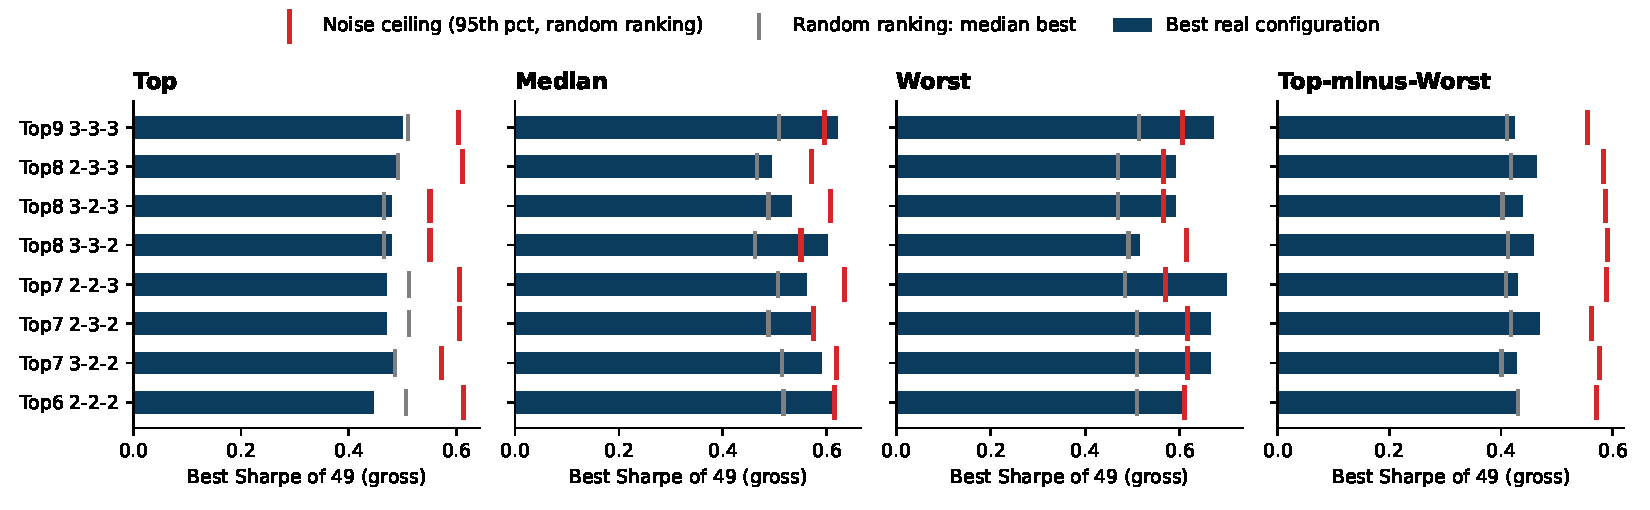
\includegraphics[width=\linewidth]{figs/fig2_noise_ceiling.pdf}
\caption{Best gross Sharpe ratio of 49 configurations in each universe split (bars) against the noise ceiling (red) and the median best Sharpe ratio under random ranking (grey).\label{fig:noise}}
\end{adjustwidth}
\end{figure}

\begin{table}[H]
\begin{adjustwidth}{-\extralength}{0cm}
\caption{Multiple-testing diagnostics over all \nConfigs{} configurations (gross). Relative performance is measured against 1/N of the same commodities at the same frequency for the long-only groups and against zero for the long--short spread. Stationary bootstrap with mean block length 21 sessions, 5000 replications. The Hansen $p$-value varies between about 0.01 and 0.03 across bootstrap seeds.\label{tab:formal}}
\small
\begin{tabularx}{\fulllength}{Xr}
\toprule
\textbf{Diagnostic} & \textbf{Value}\\
\midrule
White Reality Check $p$-value & \rcP\\
Hansen SPA $p$-value (consistent) & \spaP\\
\quad best studentised statistic (1-day reversal, Worst 3 of 7, daily) & \spaT\\
Deflated Sharpe ratio of the best configuration (must exceed 0.95) & \dsr\\
\quad annualised Sharpe of the best configuration & \dsrSr\\
\quad expected maximum annualised Sharpe of \nConfigs{} trials under the null & \dsrExpMax\\
Probability of backtest overfitting (CSCV, 16 blocks, \pboComb{} splits) & \pbo\\
\bottomrule
\end{tabularx}
\end{adjustwidth}
\end{table}



The formal diagnostics point in the same direction (Table~\ref{tab:formal}). The Reality Check does not reject the null that no configuration beats its benchmark ($p=\rcP$). Hansen's test, which removes the influence of clearly poor configurations, does reject it ($p \approx \spaP$; between 0.01 and 0.03 across bootstrap seeds), and the configuration with the largest studentised statistic (\spaT) is again the one-day reversal. The deflated Sharpe ratio of the best configuration is \dsr{} (\dsrDistinct{} counting only distinct portfolios), well below the 0.95 required, because its annualised Sharpe of \dsrSr{} barely exceeds the \dsrExpMax{} expected from the best of \nConfigs{} trials with no skill. The probability of backtest overfitting is \pbo: in about a third of the cross-validation splits, the configuration that ranks first in-sample ranks below the median out-of-sample.

\subsection{The Middle Group Is a Volatility Sort}\label{sec:median}

The middle group beats 1/N in \medBeatsEw{} of its 392 configurations, against \topBeatsEw{} for Top and \worstBeatsEw{} for Worst. The mechanism is visible in its composition. A commodity with volatile returns is more likely than a quiet one to have an extreme trailing return, in either direction, and so to land in the Top or Worst group. The middle group therefore holds the quieter commodities more often: its mean annualised volatility is \volMedian, against \volTop{} for Top and \volWorst{} for Worst. With a 21-session lookback and monthly rebalancing, natural gas is in the middle group of Top6 \ngMedSixt{} of the time and of Top9 \ngMedNine{} of the time, where a random ranking would place it one third of the time; gold is in the middle group of Top9 \goldMedNine{} of the time. In a sample in which natural gas lost 28\% a year, holding it less often is worth a great deal. Simply excluding natural gas from 1/N gives Sharpe ratios of \exNgLo{} to \exNgHi{} across universes and frequencies (\exNgSix{} for Top6), higher than the mean Sharpe ratio of the middle group in any universe (\medMeanLo{} to \medMeanHi). We therefore read the middle group as an indirect, and less effective, form of volatility screening rather than as a return anomaly. The interpretation is related to the low-risk effects documented in equities \citep{ang2006,frazzini2014} and to evidence that formation-period volatility shapes momentum portfolios \citep{fan2022}; in commodities, \citet{hollstein2021} find that idiosyncratic volatility is not priced.

\subsection{A Real but Untradeable One-Day Reversal}\label{sec:reversal}

Holding the worst performers of the previous session and rebalancing daily yields gross Sharpe ratios of \revSrLo{} to \revSrHi{} across the eight splits, stable across both halves of the sample, and is the only effect to clear the noise ceiling in most grids and to drive the rejection in Hansen's test. In practice it cannot be implemented. It turns over \revTurnLo{} to \revTurnHi{} times a year, so its Sharpe ratio falls to \revSrOneLo--\revSrOneHi{} at 1 bp, \revSrTwoLo--\revSrTwoHi{} at 2 bp and \revSrFiveLo{} to \revSrFiveHi{} at 5 bp; its excess return over Treasury bills is exhausted at \revBeCashLo{} to \revBeCashHi{} bp. A more basic problem is that the backtest ranks commodities on the closing prices of session $s$ and buys at those same closes. Table~\ref{tab:reversal} shows that holding the same portfolio from one session later reduces the Sharpe ratio from \revSixLagZero{} to \revSixLagOne{} for Top6, below that of daily 1/N, and from \revNineLagZero{} to \revNineLagOne{} for Top9, about the level of 1/N. The effect is not simply an artefact of commodities settling at different times of day: restricted to seven contracts that settle on CME Group exchanges, whose settlement times are closer together though not identical, it is still \revUsLagZero{} at the same close and \revUsLagOne{} one session later. This pattern, a reversal that exists in closing prices but is gone by the next session, is consistent with short-lived price pressure absorbed by liquidity providers \citep{kang2020}, and it contrasts with \citet{dellacorte2015}, who find no daily close-to-close reversal in their commodity sample.

\begin{table}[H]
\begin{adjustwidth}{-\extralength}{0cm}
\caption{The 1-day reversal (hold the worst performers of the previous session, rebalanced daily), gross of costs, when executed at the signal close, one session later and two sessions later. The US-settled universe keeps only contracts that settle on CME Group exchanges (WTI, natural gas, gold, silver, soybeans, corn, copper).\label{tab:reversal}}
\small
\begin{tabularx}{\fulllength}{Xrrrrrr}
\toprule
& \multicolumn{2}{c}{\textbf{Same close}} & \multicolumn{2}{c}{\textbf{One day later}} & \multicolumn{2}{c}{\textbf{Two days later}}\\
\textbf{Universe, holding} & \textbf{Sharpe} & \textbf{USD 100 $\to$} & \textbf{Sharpe} & \textbf{USD 100 $\to$} & \textbf{Sharpe} & \textbf{USD 100 $\to$}\\
\midrule
Top 6, worst 2 & 0.61 & 3,645 & 0.16 & 111 & 0.22 & 171\\
Top 7, worst 2 & 0.67 & 5,117 & 0.16 & 111 & 0.19 & 134\\
Top 7, worst 3 & 0.70 & 4,033 & 0.27 & 257 & 0.20 & 161\\
Top 9, worst 3 & 0.67 & 3,365 & 0.34 & 389 & 0.16 & 129\\
US-settled 7, worst 2 & 0.55 & 1,851 & 0.16 & 113 & -- & --\\
\bottomrule
\end{tabularx}
\end{adjustwidth}
\end{table}



\subsection{Rebalance-Date Luck}

The best configuration net of costs, the middle two of Top6 with a 21-session lookback rebalanced at each year-end, turns USD 100 into USD \starDec{} with a Sharpe ratio of \starSrDec. Figure~\ref{fig:month} reruns the identical rule with each of the other eleven month-ends as the annual rebalance date. The terminal values range from USD \starMin{} to USD \starMaxOther{}, with a median across all twelve dates of USD \starMedian{}, and the Sharpe ratios from \starSrMin{} to \starSrMaxOther{} (mean \starSrOtherMean{} over the eleven other dates). December is the best of the twelve. These values are before costs; at 1 bp the year-end version ends at USD \starDecOne{} and the others at USD \starMinOne{} to USD \starMaxOne. An investor in 2001 had no way of knowing which month-end would turn out to be the luckiest; only the full sample reveals it.

\begin{figure}[H]
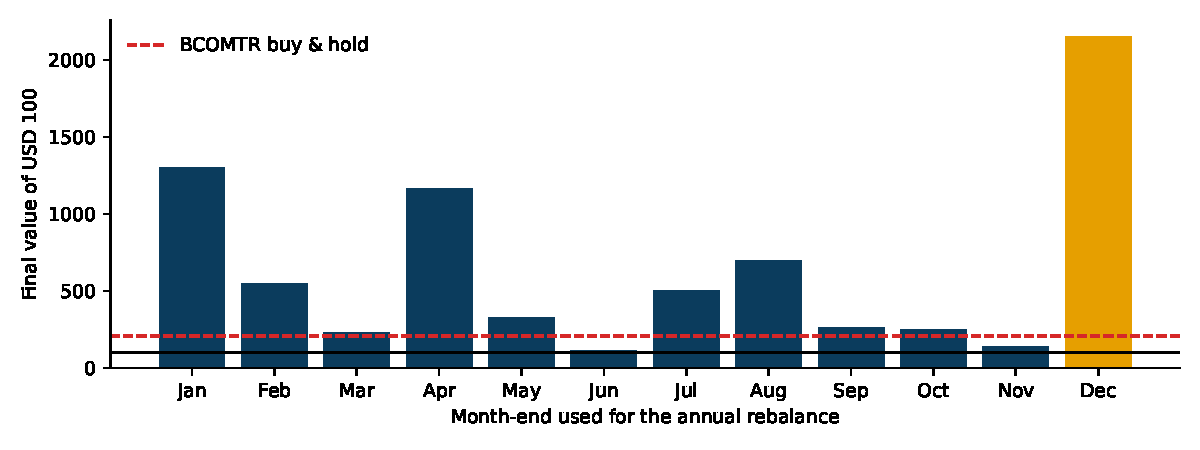
\includegraphics[width=\textwidth]{figs/fig4_rebalance_month.pdf}
\caption{Terminal value of USD 100 for the middle two of Top6 (21-session lookback) rebalanced once a year, by the month-end used for the rebalance. The year-end version is highlighted; the dashed line is BCOMTR buy-and-hold.\label{fig:month}}
\end{figure}

The effect is not confined to one rule. Across all annual configurations, the median range of Sharpe ratios across the twelve possible rebalance months is \luckAnnRange; for semiannual configurations across six offsets it is \luckSemiRange{} and for quarterly across three offsets \luckQRange. Even biweekly rebalancing is exposed: switching to the other set of alternate weeks changes the Sharpe ratio by a median of \luckBwRange, and the biweekly configuration in Table~\ref{tab:bestfreq} ends at USD \bwAlt{} (Sharpe \bwAltSr) instead of USD \bwGrid. The calendar year-end is the best of the twelve dates for only \luckAnnCalBest{} of annual configurations, but it is the best date for \topAnnFirst{} of the \topAnnN{} annual configurations with the highest year-end Sharpe ratio, and among the best \topAnnWorstRank{} dates for all of them: in other words, selecting the best annual configuration largely means selecting a lucky date as well.

\subsection{Out-of-Sample Selection}

Table~\ref{tab:wf} and Figure~\ref{fig:wf} report the most direct test. The five configurations with the highest gross Sharpe ratio over 2001--2013 (\wfInLo{} to \wfInHi) achieve Sharpe ratios of \wfOutHi{} or less over 2014--2026 and turn USD 100 into USD \wfFinLo{} to USD \wfFinHi, ranking between \wfRankLo{} and \wfRankHi{} of \nConfigs{} configurations; buy-and-hold turned USD 100 into USD \wfBhFinal{} over the same period. The in-sample leaders are all momentum portfolios (three long--short spreads and two Top groups) with a five-day lookback and semiannual rebalancing, families that do not exceed their noise ceilings over the full sample either. Reselecting the best configuration at the end of each year and holding it over 2006--2026 turns USD 100 into USD \wfaFinG{} before costs (Sharpe \wfaSrG), against USD \wfaBh{} for buy-and-hold over the same years; at 2 bp it ends at USD \wfaFinN.

\begin{table}[H]
\begin{adjustwidth}{-\extralength}{0cm}
\caption{Out-of-sample check. The five configurations with the highest gross Sharpe ratio over 2001--2013, run unchanged over 2014--2026. Rank is out of \nConfigs{} on the out-of-sample period. BCOMTR buy-and-hold over 2014--2026: USD 100 $\to$ \wfBhFinal, Sharpe \wfBhSr.\label{tab:wf}}
\small
\begin{tabularx}{\fulllength}{Xrrrr}
\toprule
\textbf{Configuration (rebalance)} & \textbf{Sharpe 2001--13} & \textbf{Sharpe 2014--26} & \textbf{USD 100 $\to$} & \textbf{Rank 2014--26}\\
\midrule
Best 2 $-$ Worst 3 of 8 (2-3-3), 5d (semiannual) & 0.92 & 0.08 & 71 & 1,005\\
Best 3 $-$ Worst 3 of 9 (3-3-3), 5d (semiannual) & 0.90 & 0.00 & 60 & 1,222\\
Best 3 of 9 (3-3-3), 5d (semiannual) & 0.88 & 0.11 & 97 & 910\\
Best 2 $-$ Worst 3 of 7 (2-2-3), 5d (semiannual) & 0.86 & 0.06 & 65 & 1,058\\
Best 2 of 7 (2-3-2), 5d (semiannual) & 0.86 & 0.12 & 93 & 837\\
\bottomrule
\end{tabularx}
\end{adjustwidth}
\end{table}



\begin{figure}[H]
\begin{adjustwidth}{-\extralength}{0cm}
\centering
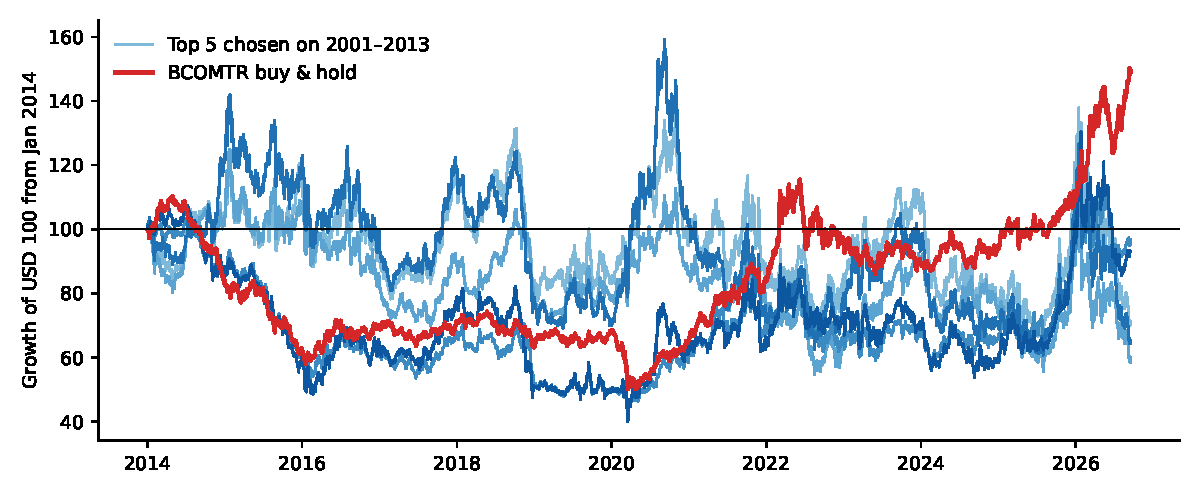
\includegraphics[width=\linewidth]{figs/fig5_walk_forward.pdf}
\caption{Growth of USD 100 from January 2014 for the five configurations with the highest gross Sharpe ratio over 2001--2013 (blue), against BCOMTR buy-and-hold (red).\label{fig:wf}}
\end{adjustwidth}
\end{figure}

\subsection{Data Quality of Generic Futures Prices}

The companion study \citep{meena2026} showed that a free data source recorded opening prices at the session low far more often than at the high, which manufactured an overnight anomaly, and that an exact binomial test on the position of the open within the day's range detects the defect without a second data source. We apply the same screen to every daily open, high, low and close (OHLC) series we hold (Table~\ref{tab:screen}). It reproduces the defect in the free DXY series (\scrFreeLow{} opens at the low against \scrFreeHigh{} at the high) and passes the exchange-sourced DXY futures used as the control in that study (\scrDxLow{} against \scrDxHigh, $p=\scrDxP$). Among the \scrNBloom{} Bloomberg generic contracts, energy and precious metals pass, but \scrNFail{} are flagged: the five London Metal Exchange (LME) contracts record 6.6\% to 8.4\% of opens outside the day's own high--low range, almost all of them before 2012 (\lmePreLo\% to \lmePreHi\% of sessions before 2012 and essentially none after); corn, soybeans and coffee show asymmetric opens that are strongest before 2012; and Kansas wheat is flagged for opens outside the range (\kwPre\% of sessions before 2012, none after). These flags do not affect our results, which use only closing values of total-return indices, but they rule out using these generic OHLC series for any open-based decomposition without further cleaning.

\begin{table}[H]
\begin{adjustwidth}{-\extralength}{0cm}
\caption{Open-location screen on daily OHLC data. Under an unbiased open, P(open = low) = P(open = high); $p$ is the exact two-sided binomial test. ``Pos.'' is the mean position of the open in the day's range (0.5 expected); ``Outside'' is the share of opens outside the day's own range. Flag = FAIL if $p$ is below 0.01 after Bonferroni correction over all 37 series screened, or more than 1\% of opens lie outside the range. Selected rows; all 30 Bloomberg contracts are in the replication files.\label{tab:screen}}
\small
\begin{tabularx}{\fulllength}{Xlrrrrrl}
\toprule
\textbf{Series} & \textbf{Source} & \textbf{Open=low} & \textbf{Open=high} & \textbf{$p$} & \textbf{Pos.} & \textbf{Outside} & \textbf{Flag}\\
\midrule
Corn (C 1) & Bloomberg & 443 & 326 & 2.8e-05 & 0.48 & 0.1\% & FAIL\\
WTI Crude Oil (CL1) & Bloomberg & 126 & 115 & 0.520 & 0.50 & 0.1\% & pass\\
Brent Crude Oil (CO1) & Bloomberg & 218 & 207 & 0.628 & 0.50 & 0.0\% & pass\\
Gold (GC1) & Bloomberg & 577 & 545 & 0.355 & 0.50 & 0.2\% & pass\\
Copper (HG1) & Bloomberg & 605 & 561 & 0.208 & 0.50 & 0.3\% & pass\\
Coffee (KC1) & Bloomberg & 704 & 896 & 1.7e-06 & 0.52 & 0.3\% & FAIL\\
Wheat (Kansas HRW) (KW1) & Bloomberg & 653 & 557 & 0.006 & 0.49 & 1.5\% & FAIL\\
Aluminium (LA1) & Bloomberg & 1266 & 1315 & 0.345 & $-$1.46 & 7.0\% & FAIL\\
Nickel (LN1) & Bloomberg & 1727 & 1366 & 9.2e-11 & $-$2.03 & 7.7\% & FAIL\\
Natural Gas (NG1) & Bloomberg & 119 & 152 & 0.052 & 0.51 & 0.8\% & pass\\
Soybeans (S 1) & Bloomberg & 499 & 319 & 3.3e-10 & 0.46 & 0.1\% & FAIL\\
Silver (SI1) & Bloomberg & 656 & 603 & 0.143 & 0.50 & 0.3\% & pass\\
U.S. Dollar Index futures (DX) & Barchart (exch.) & 64 & 60 & 0.788 & 0.50 & 0.0\% & pass\\
U.S. Dollar Index (free provider) & Free provider & 204 & 82 & 3.7e-13 & 0.48 & 0.0\% & FAIL\\
\bottomrule
\end{tabularx}
\end{adjustwidth}
\end{table}



\section{Discussion}\label{sec:discussion}

\subsection{Implications for Investors}

Every configuration in Table~\ref{tab:bestfreq} beats buy-and-hold in the backtest before costs, and each one fails for a different reason that the backtest by itself does not reveal. The daily reversal earns its returns at closing prices that cannot be traded. The slow middle-group rules are volatility screens that happened to exclude the worst commodity of the period, and the best of them also owes its rank to the calendar. The momentum spreads that led in the first half of the sample did not persist into the second. None of these problems shows up in the Sharpe ratio, drawdown or $t$-statistic of the winning configuration. They appear only when that configuration is compared with what the whole search, the next session, another rebalance date or the following decade would have produced.

The practical lesson is easy to apply. A backtest of a cross-sectional commodity rule should report the number of configurations tried, a benchmark of the same commodities at equal weight, net results at a realistic cost, the result with a one-session delay, and the spread of results across rebalance dates. For small universes, a noise ceiling of the kind used here is cheap to compute and easy to explain, because it answers a simple question: how good would the best result look if the signal carried no information?

\subsection{Limitations}\label{sec:limits}

The universe is small by design, so a group of two or three commodities is close to single-commodity selection, and results for broader universes may differ. The universe was chosen using liquidity measured over the whole sample. The cost model is linear and ignores market impact, the bid--ask spread varies across commodities and over time, and total-return sub-indices are themselves a construction: replicating them requires rolling futures, which adds costs we do not model. The noise ceiling uses 200 replications, so verdicts within about 0.01 of the ceiling (three of the 32 grids in Table~\ref{tab:noise}) are within simulation error, and the Hansen test $p$-value varies between about 0.01 and 0.03 across bootstrap seeds. Finally, the null results are specific to price-based ranking; signals built from the futures curve or from trader positions \citep{koijen2018,kang2020} are not tested.

\section{Conclusions}

On investable total-return data for the most liquid commodities, a declared search over \nConfigs{} cross-sectional configurations produces several backtests that beat buy-and-hold by a wide margin. None of them survives the checks an investor would need to apply before trading. Momentum does no better than random rankings, the middle group's advantage comes from a volatility screen that mostly avoids natural gas, the one-day reversal disappears with a one-session delay and a few basis points of cost, the best net configuration depends on its rebalance date, and the in-sample leaders trail buy-and-hold out of sample. The tools that expose these failures (a noise ceiling, an execution delay, a rebalance-date sweep and out-of-sample selection) are simple to apply, and we suggest that they be reported alongside any cross-sectional commodity backtest.

\vspace{6pt}

\authorcontributions{Conceptualization, E.P. and A.M.; methodology, A.M. and E.P.; software, A.M.; validation, A.M.; formal analysis, A.M.; data curation, A.M.; writing---original draft preparation, A.M.; writing---review and editing, E.P. and A.M.; supervision, E.P. All authors have read and agreed to the published version of the manuscript.}

\funding{This research received no external funding.}

\dataavailability{Restrictions apply to the availability of these data. Data were obtained from Bloomberg L.P. and are available from Bloomberg with its permission; the tickers (the BCOM total-return sub-indices in Table~\ref{tab:assets}, the generic first contracts and BCOMTR) and the retrieval period are given in the text. The Treasury bill rate is public (FRED series DTB3). Code that reproduces every table and figure from a Bloomberg export is available from the authors and will be deposited in a public repository upon acceptance. The replication code for the companion study is available at \url{https://github.com/RyanSingh0/dxy-fx-strategies}.}

\acknowledgments{The authors thank Boston University Libraries for Bloomberg terminal access. During the preparation of this study, the authors used Claude (Anthropic) to help write and debug parts of the analysis code, to check the study against recent literature in the field, and to correct language and consistency in the manuscript. The authors reviewed and verified all outputs and take full responsibility for the content of this publication.}

\conflictsofinterest{The authors declare no conflicts of interest.}

\abbreviations{Abbreviations}{
The following abbreviations are used in this manuscript:\\

\noindent
\begin{tabular}{@{}ll}
BCOM & Bloomberg Commodity Index\\
BCOMTR & Bloomberg Commodity Index Total Return\\
bp & basis point\\
CSCV & combinatorially symmetric cross-validation\\
DXY & U.S. Dollar Index\\
FRED & Federal Reserve Economic Data\\
LIBOR & London Interbank Offered Rate\\
LME & London Metal Exchange\\
OHLC & open, high, low, close\\
SPA & superior predictive ability\\
WTI & West Texas Intermediate
\end{tabular}
}

\begin{adjustwidth}{-\extralength}{0cm}
\reftitle{References}
\bibliography{refs}
\PublishersNote{}
\end{adjustwidth}
\end{document}
